\documentclass[a4paper, 12pt, oneside]{extreport}
\input{$HOME/Templates/lpnu_doc_templates/settings/preamble}
\usepackage{etoolbox} % пакунок для розширеного програмування
%xelatex

\newtoggle{Report}
\togglefalse{Report}

\newtoggle{RGR}
\togglefalse{RGR}

\newcommand\Type{Пояснювальна записка}
\newcommand\Number{}
\newcommand\Discipline{Комп'ютерна схемотехніка та архітектура комп'ютерних систем}
\newcommand\Topic{Розрахунок і побудова блоку пам'яті}

\newcommand\Class{студент групи \Group}
\newcommand\Author{\Lname~\Initials}
\newcommand\Position{доцент}
\newcommand\Instructor{Чкалов О. В.}
\newcommand\Variant{12}

\usepackage[ukrainian]{nomencl}
\usepackage{array, booktabs}
\addbibresource{~/Documents/uni/bibliography.bib}
\usepackage{csvsimple}
\usepackage{pgfplotstable}
\usepackage{hyperref}

% \renewcommand{\nomlabel}[1]{\hfil #1\hfil}
\renewcommand{\nomlabel}[1]{\emph{#1}}
\makenomenclature

\nomenclature{ОЗП}{Оперативний запам'ятовувальний пристрій}
\nomenclature{ЗП}{запам'ятовувальний пристрій}
\nomenclature{ВІС}{велика інтегральна мікросхема}
\nomenclature{СДНФ}{скорочена диз’юнктивна нормальна форма}
\nomenclature{СКНФ}{скорочена кон’юнктивна нормальна форма}
\nomenclature{ШК}{шина керування – призначена для передачі сигналів керування, обліку, запитів на переривання, передачі керування, синхронізації і т. д. }
\nomenclature{ША}{шина адрес – призначена для пересилки кодів адресної інформації до оперативної пам’яті або електронних модулів комп’ютера, для доступу до комірок пам’яті або пристроїв вводу-виводу}
\nomenclature{ШД}{шина даних – призначена для передачі даних між електронними модулями комп’ютера}
\nomenclature{WE}{вхід дозволу для запису (Write enable)}
\nomenclature{CS}{вибір кристалу(Chip select); доступ до однієї з мікросхем, яка входить у пристрій.}
\nomenclature{МПС}{Мікропроцесорна система}
% makeindex Мілюхін_ПП-14_1_ргр_пояснювальна.nlo -s nomencl.ist -o Мілюхін_ПП-14_1_ргр_пояснювальна.nls

\begin{document}

\newgeometry{top=1cm,bottom=1cm,right=1.5cm,left=1.5cm}
\newcommand{\LINE}{\rule{\linewidth}{0.4mm}}
\begin{titlepage}
	\center

	\textsc{МІНІСТЕРСТВО ОСВІТИ І НАУКИ УКРАЇНИ}\\
	\textsc{НАЦІОНАЛЬНИЙ УНІВЕРСИТЕТ "`ЛЬВІВСЬКА ПОЛІТЕХНІКА"'}\\
	% \textsc{національний університет ``львівська політехніка''}\\
	\small
	\iftoggle{RGR} {}
	{
		{\Institute}\\
	}
	{кафедра \Department}\\
	[1.5cm]
	\normalsize
	%\large

	\includegraphics[scale=0.35]{$HOME/Templates/lpnu_doc_templates/lpnu_logo.png}\\[1.5cm]

	\iftoggle{Report}
	{
		\textsc{\LARGE\bfseries звіт}\\
		\textsc{ до \Type \, \No\Number}\\
	}
	{
		\textsc{\LARGE\bfseries \Type~\Number}\\
	}
до розрахунково-графічної роботи \\
  з дисципліни: "`\Discipline"'\\
  %на тему: \\

	\iftoggle{RGR}
	{
	\LINE\\[0.2cm] % норм?
	\large
		\textsc{\bfseries Варіант \Variant}\\[0cm]
	\LINE\\[1cm]
	}
	{
	\LINE\\[0.2cm]
	\large
	\textsc{\bfseries \Topic}\\[0cm]
	\normalsize
	\LINE\\[1cm]
	}


	\begin{flushright}
		\large
		\textit{Виконав}\\
		\normalsize
		\Class \; \textsc{\Author}

		\large
		\textit{Перевірив(ла)}\\
		\normalsize
		\Position \; \textsc{\Instructor}
	\end{flushright}

	\vfill
	Львів	\the\year{}
\end{titlepage}
\Margins


\chapter*{Індивідуальне завдання}
\addcontentsline{toc}{chapter}{Індивідуальне завдання}

Потрібно розробити блок пам'яті вказаного типу, об'єму та розрядності,
на основі мікросхем заданих об'єму та розрядності. Моя конфігурація
наведена в таблиці нижче.

\begin{table}[h]
\begin{tabular}{lr}
	Тип пам’яті & ОЗП \\
	Об’єм & 2Кх1   \\
	Конф. м/с & 1Кх1 \\
\end{tabular}
\end{table}

\printnomenclature

\tableofcontents

\chapter*{Вступ}
\addcontentsline{toc}{chapter}{Вступ}

% Тут необхідно відобразити актуальність розробки блоку пам’яті,
% перспективність застосування пам'яті в мікропроцесорних системах,
% загальний підхід до розв’язку  поставленої задачі.

МПС використовуються в різних галузях, від особистих комп'ютерів до вбудованих
систем в автомобілях, мобільних пристроях та промислових контролерах. Одним із
ключових елементів таких систем є блок пам'яті, який забезпечує зберігання та
доступ до великих обсягів даних. Розробка ефективних та надійних блоків пам'яті
для мікропроцесорів є актуальною проблемою у сучасній електроніці.

\section*{Актуальність розробки блоку пам'яті}

Актуальність розробки блоку пам'яті полягає в постійному зростанні потреб у
більш високій ємності та швидкості доступу до даних. Завдяки розвитку
технологій виготовлення напівпровідникових пристроїв, сьогодні ми можемо
розробляти мікросхеми зі значно більшою ємністю пам'яті та швидшим доступом до
неї. Але вони складні в організації, тому наше завдання полягає в розробці значно
простішого блоку пам'яті для процесора КР580ВМ80, щоб зрозуміти основні принципи.

\section*{Перспективність застосування пам'яті в МПС}

Застосування пам'яті в МПС виявляє безліч перспектив. Від персональних
комп'ютерів, де використовуються швидкі ОЗП для
запуску програм та зберігання даних, до вбудованих систем, де
використовуються низькопотужні та енергоефективні флеш-пам'яті для
зберігання програмного забезпечення та конфігураційних даних.

% Пристрої, з якими ми щодня взаємодіємо, використовують
% мікропроцесори та вбудовані системи з різними видами
% пам'яті для забезпечення їхньої
% роботи. Наприклад, мобільні пристрої використовують флеш-пам'ять
% для зберігання операційної системи, додатків та користувацьких
% даних, тоді як автомобілі мають спеціалізовані пам'яті для
% зберігання конфігураційних даних, журналів подій та інших важливих
% відомостей.

\section*{Загальний підхід до розв'язку поставленої задачі}

Загальний підхід до розв'язання поставленої задачі передбачає
аналіз вимог щодо ємності, швидкості та надійності пам'яті для
конкретної МПС. На основі цього аналізу розробляються алгоритми та
архітектура блоку пам'яті, що задовольняють ці вимоги. Потім
проводиться детальне проектування та оптимізація блоку пам'яті.

Конкретно в цій роботі потрібно:

\begin{enumerate}
\item{Вибрати тип мікросхеми для побудови блоку та обґрунтувати свій вибір}
\item{Виділити адресний простір для блоку пам'яті}
\item{Визначити кількість мікросхем пам'яті для блоку}
\item{Синтезувати схему дешифратора адрес для блоку пам'яті}
\end{enumerate}

% Після завершення розробки проводяться тестування та
% верифікація блоку пам'яті для забезпечення його коректної роботи в
% реальних умовах.

% Оскільки розробка ефективних та потужних блоків пам'яті є важливим
% завданням у сфері мікропроцесорних систем, в подальшому дослідженні
% та розвитку цієї області приділяється значна увага. Результати
% таких досліджень допоможуть створити ще більш продуктивні та
% надійні мікропроцесорні системи, що забезпечать подальше розширення
% можливостей сучасної електроніки.

% 1) закріплення і узагальнення знань, отриманих студентом на
% лекційних, лабораторних і практичних заняттях, застосування цих знань до
% комплексного вирішення конкретної інженерної задачі;

% 2) застосування формалізованих методів аналізу і синтезу цифрових схем;

% 3) мінімізація складу елементів;

% 4) оптимальний вибір сучасних інтегральних мікросхем різного
% ступеню інтеграції;

% 5) забезпечення електричних режимів роботи інтегральних мікросхем;

% 6) дотримання вимог чинних нормативно - технічних вимог при
% оформленні результатів виконання РГР.

\chapter{Вибір і обґрунтування типу мікросхеми для побудови блоку пам'яті}

\section{Вибір мікросхеми}

Мені потрібно було побудувати блок 2Kx1 на базі мікросхем організації 1Kx1.
Отже, згідно з варіантом завдання я підібрав мікросхему, спираючись найбільше
на її швидкодію. Зупинився на К1500РУ415, яку знайшов у \parencite[ст. 485]{nefedov9}.

\section{Характеристика мікросхеми}

ОЗП місткістю 1024 (1024x1) бітів. Корпус типу 4112.16-9, маса не перевищує 1 г.

% \begin{table}
% 	\begin{tabular}{ll}
% К	&мікросхема призначена для широкого застосування;  \\
% М	&металокерамічний, керамічний або склокерамічний корпус з паралельним \\
% 	&дворядним розташуванням виводів(другого типу);  \\
% 1	&група мікросхеми по конструктивно-технологічному признаку  (напівпровідникова); \\
% 85	&порядковий номер розробки серії;  \\
% РУ	&ОЗП;  \\
% 7	&порядковий номер розробки серії 185
% 	\end{tabular}
% \end{table}

\begin{figure}[h]
	\centering
	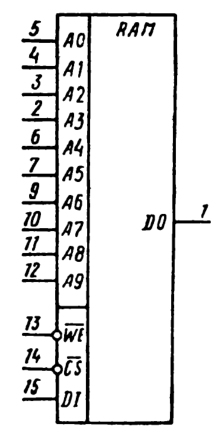
\includegraphics[width=.18\textwidth]{k1500py415.png}
	\caption{умовне позначення К1500РУ415}
\end{figure}

\newcommand\chip{К1500РУ415}

\section{Призначення виводів}

\begin{table}[h]
	\centering
	\begin{tabular}{r|l}
	2--7, 9--12	&адресні входи вибору стрічок \\
	13	&інверсний вхід дозволу запису \\
	14	&інверсний вхід вибірки мікросхеми \\
	15	&вхід інформації 1-го розряду \\
	1	&вихід інформації 1-го розряду
	\end{tabular}
	\caption{призначення виходів \chip}
\end{table}

\section{Електричні характеристики}

\newcommand\myheading[1]{\hspace{-1em}\textbf{#1}\\}

% \textcite{nefedov9}
% \parencite{nefedov9}

\begin{table}[h] % якась дупа
	% \begin{tabular}{W{l}{7cm} <{\dotfill} @{}l}
	\centering
	\begin{tabular}{lr}
		% \toprule
		Номінальна напруга живлення & $-4.5$ В$\pm5\%$ \\
		Напруга низького рівня & $-1.81...-1.62$ В \\
		Напруга високого рівня & $-1.025...-0.88$ В \\
		Струм споживання & $\leq |-150|$ мА \\
\\
	\myheading{Вхідний струм низького рівня}
	% \begin{tabular}{W{l}{7cm} <{\dotfill} @{}l}
		на входах $A_0$--$A_9, D_1, \overline{WR}$ & $\leq |-50|$ мкА \\
		на вході $\overline{CS}$ & $\geq0,5$ мкА \\
	\myheading{Вхідний струм високого рівня}
	% \begin{tabular}{W{l}{7cm} <{\dotfill} @{}l}
		на входах $A_0$--$A_9, D_1, \overline{WR}$ & $\leq 50$ мкА \\
		на вході $\overline{CS}$ & $\geq220$ мкА \\
\\
	% \begin{tabular}{W{l}{7cm} <{\dotfill} @{}l}
		питома споживча потужність & $\leq0.66$ мВт/біт \\
		час вибору адреси & $\leq20$ нс \\
		% \bottomrule
	\end{tabular}
	\caption{Електричні характеристики \chip}
	%\label{}
\end{table}

\chapter{Виділення адресного простору для блоку пам'яті}

% пропустити все крім озп

		В адресний простір МП КР580ВМ80 входить 64К адрес пам'яті ($2^{16}$), що
визначається 16 - розрядною адресною шиною. Мікропроцесор КР580ВМ80
може здійснювати синхронний і асинхронний обмін інформацією за даними
адресами з пам'яттю (ПЗП, ОЗП) та зовнішніми пристроями. При обробці
інформації МП зчитує коди команд з ПЗП, а дані зчитує або записує в ОЗП або
виконує обмін інформації з пам'яттю та регістрами РЗК.

\begin{table}[htbp]
	\begin{center}
		\begin{tabular}{c|c}
			0000h &  \\
			$\vdots$ & ВП \\
			0040h & \\
			% $\vdots$ & ПЗП \\
			% 1000h & \hrulefill \\
			$\vdots$ & $\vdots$ \\
			F800h & \\
			$\vdots$ & ОЗП \\
			FFFFh &
		\end{tabular}
		\caption{виділення простору адрес для ОЗП 2Kx1}
		%\label{}
	\end{center}
\end{table}

Виділимо блоку ОЗП
		простір від F800 до FFFF
		(1111 1000 0000 0000 до 1111 1111 1111 1111).

\chapter{Визначення кількості мікросхем пам'яті для блоку}

Нагадаю, що нам потрібен блок \textbf{2Kx1} із мікросхем \textbf{1Kx1}.

Нехай число комірок пам’яті блоку --- $M$, а $m$ --- об’єм пам'яті однієї мікросхеми,
тоді загальне число мікросхем, які необхідно об'єднати визначається:
$$
		L=\frac{M}{m}=\frac{2}{1}=2
		% \text{(необхідно об'єднувати послідовно).}
$$
Загальне число мікросхем, яке необхідне для реалізації блоку пам’яті
визначається , як  $P=K\cdot L$, де $P$ - загальна кількість мікросхем, а $K$ ---
кількість мікросхем для нарощення розрядності (тут $1$).

$$
	P=1\cdot 2 = 2
$$

Потрібно використати дві мікросхеми.

\chapter{Синтез схеми дешифратора адрес для блоку пам'яті}

Для адресного розподілу окремих мікросхем використовуються адресні
дешифратори (АДш), число виходів яких рівне L числу мікросхем, а число
входів визначається за заданим об'ємом та виділеним простором адрес для блоку
пам'яті. Синтез схеми адресного дешифратора складається з послідовних етапів:

\begin{enumerate}
\item табличного задання початкової та кінцевої адреси для заданого блоку
пам'яті;
\item представлення логічних виразів у СДНФ або СКНФ на основі таблиці;
\item побудова комбінаційної схеми адресного дешифратора на основі логічного
виразу.
\end{enumerate}

\section{табличне задання початкової та кінцевої адреси для заданого блоку}

\setlength{\tabcolsep}{3pt}
\begin{table}[h]
	\centering
	\csvautotabular{table.csv}
	\caption{банк 1}
	%\label{}
\end{table}

\begin{table}[h]
	\centering
	\csvautotabular{bank2.csv}
	\caption{банк 2}
\end{table}

% \pgfplotstabletypeset[
%     col sep=comma,
%     string type,
%     every head row/.style={%
%         after row=\hline
%     },
%     every last row/.style={after row=\hline},
%     columns/name/.style={column name=Name, column type=l},
%     columns/surname/.style={column name=Surname, column type=l},
%     columns/age/.style={column name=Age, column type=c},
%     ]{table.csv}

\section{представлення логічних виразів у СДНФ або СКНФ на основі таблиці}

Я побудував СКНФ, та застосувавши закони де Моргана отримав:

\begin{align}
	CS_0=
	\overline A_{15}
	+\overline A_{14}
	+\overline A_{13}
	+\overline A_{12}
	+\overline A_{11}
	+ A_{10}
	=
	\overline
	{
		A_{15}
		\cdots
		A_{11}
	}
	+ A_{10}
	\\
	CS_1=
	\overline A_{15}
	+\overline A_{14}
	+\overline A_{13}
	+\overline A_{12}
	+\overline A_{11}
	+\overline A_{10}
	=
	\overline
	{
		A_{15}
		\cdots
		A_{11}
	}
	+\overline A_{10}
\end{align}

\section{побудова комбінаційної схеми адресного дешифратора на основі логічного виразу}

Для побудови схеми потрібно:

\begin{itemize}
	\item 1 елемент НЕ-І на 5 входів
	\item 1 елемент НЕ-ЧИ з одним входом
	\item 2 елементи ЧИ на 2 входи
\end{itemize}

\begin{figure}[h]
	\centering
	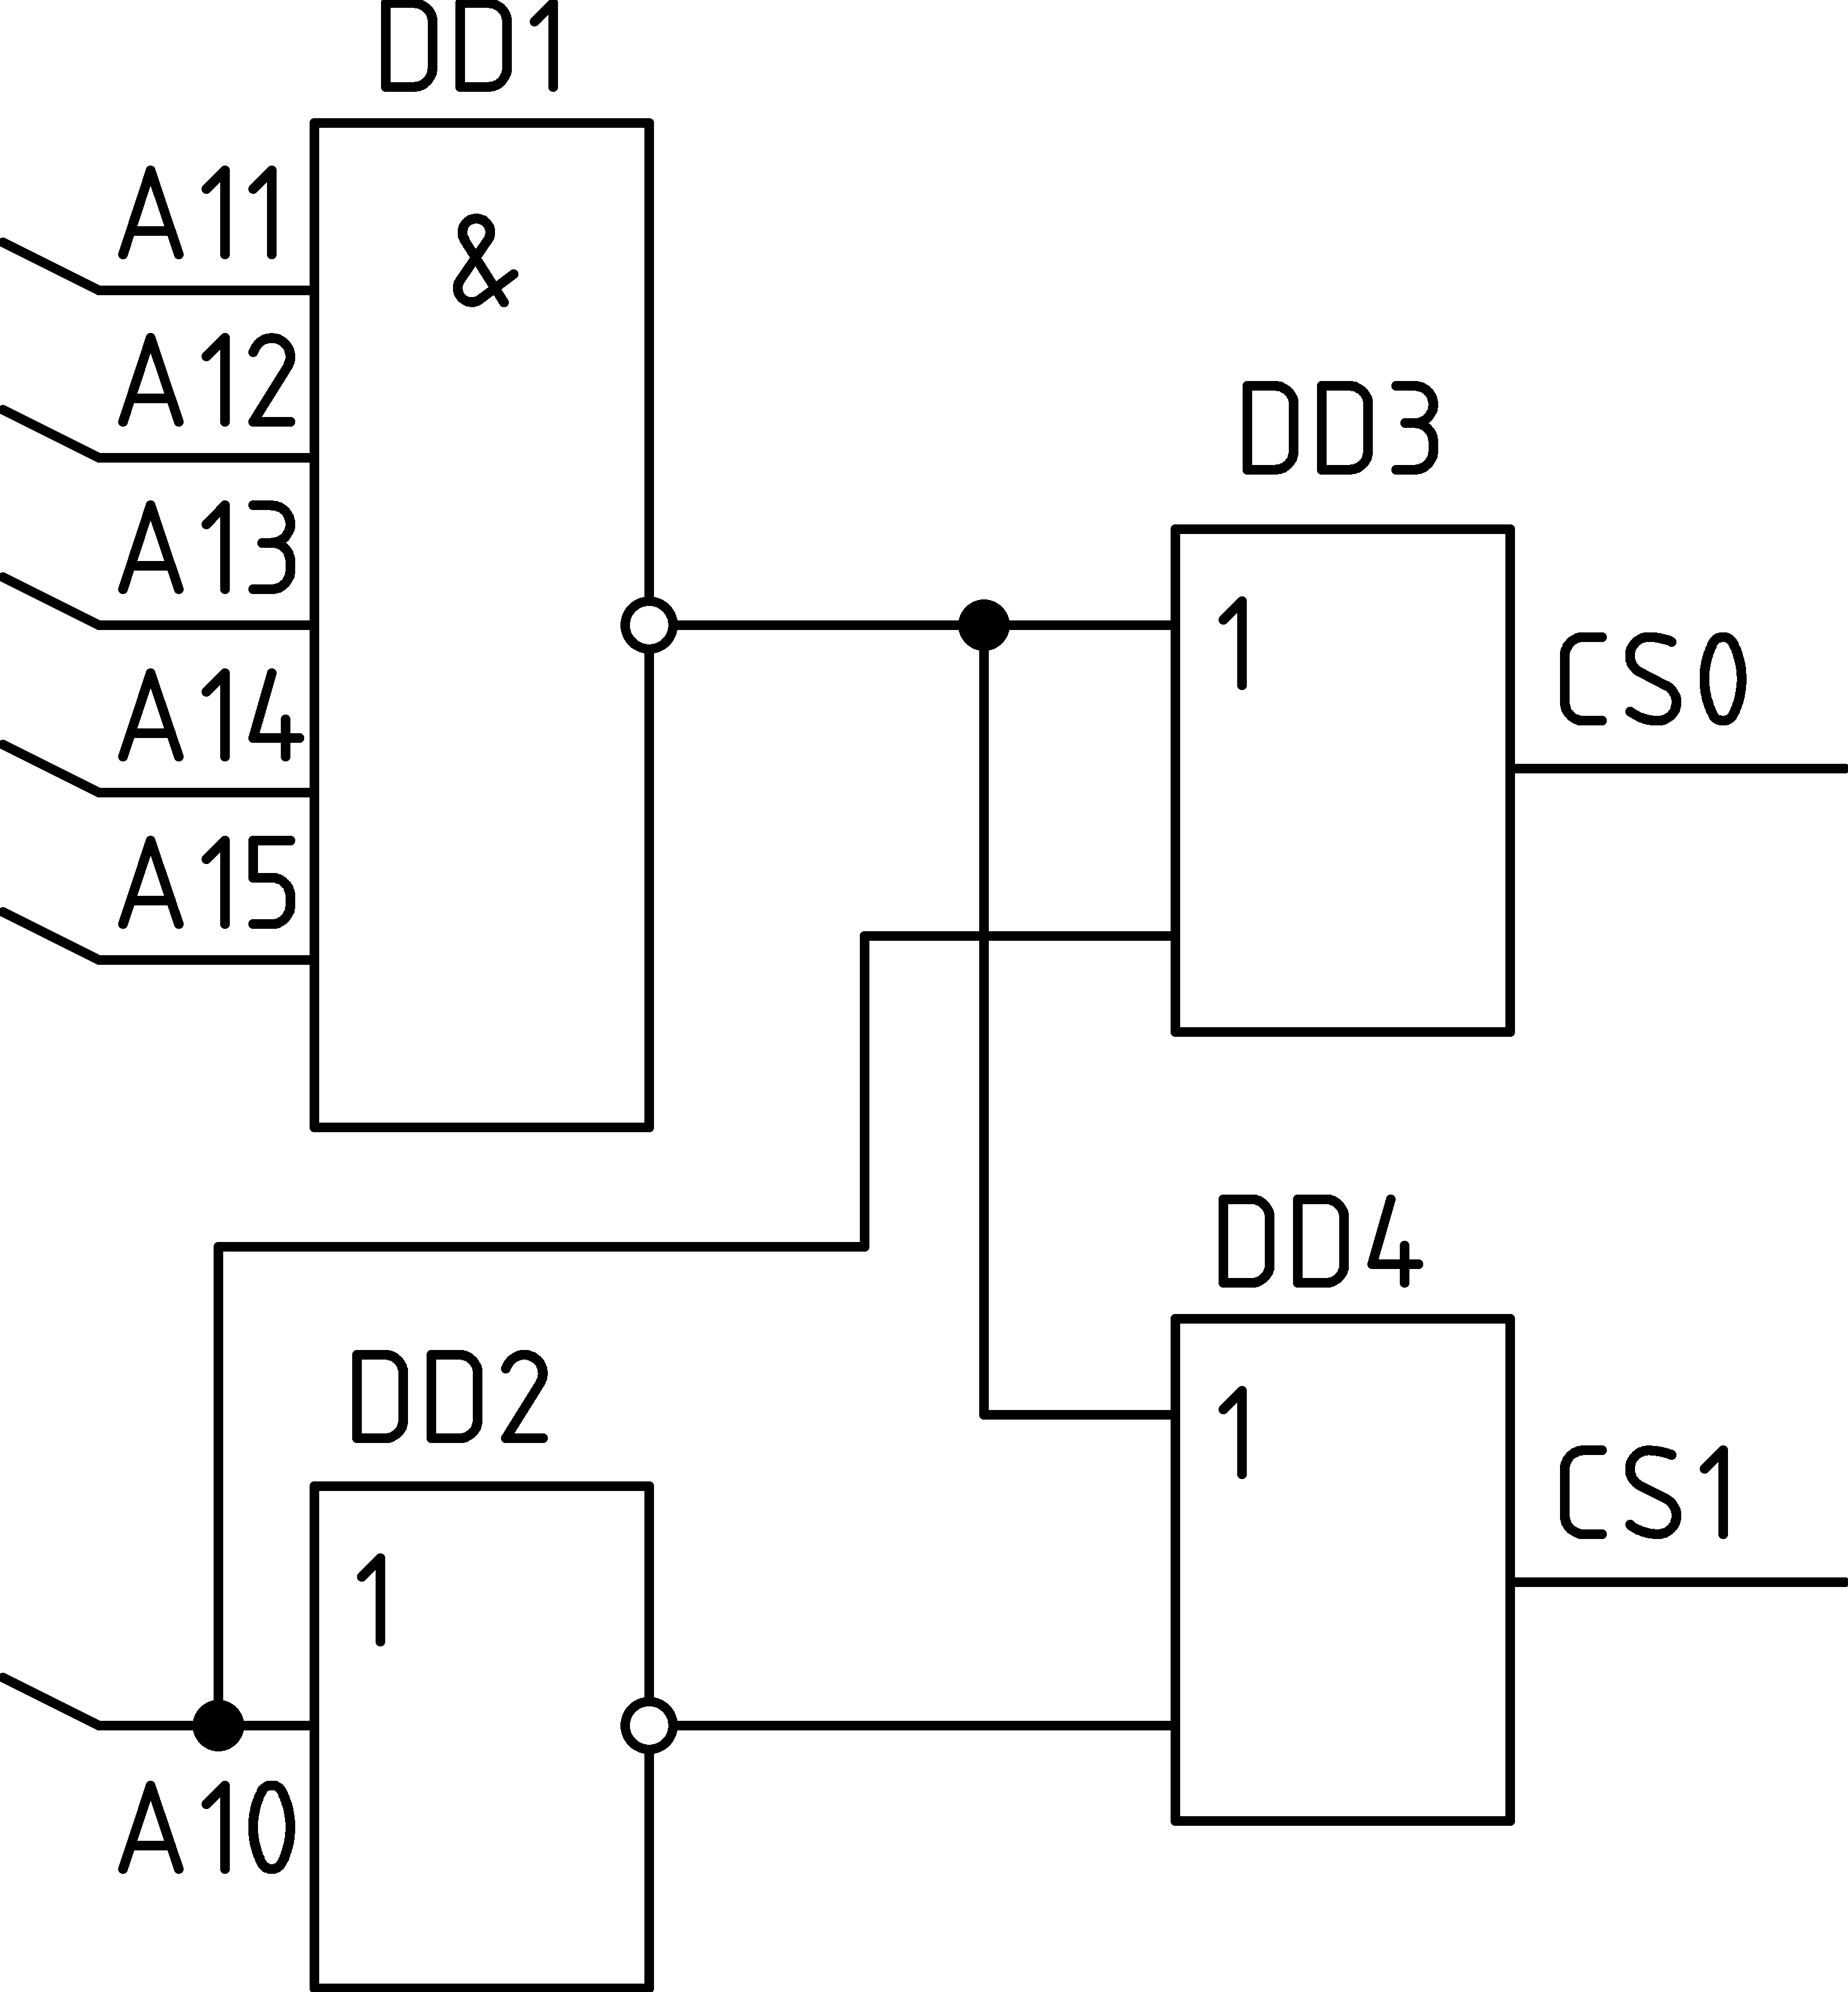
\includegraphics[width=.3\textwidth]{decoder}
	\caption{схема адресного дешифратора}
\end{figure}

\chapter*{Аналіз результатів та висновки}
\addcontentsline{toc}{chapter}{Аналіз результатів та висновки}

В цій роботі я набув досвіду проєктування блоку пам'яті
(якщо точніше, то ОЗП) для процесора КР580ВМ80.
Навчився підбирати потрібні мікросхеми та переносити
їх на креслення, будувати дешифратор для визначення
банків, які потрібно використовувати залежно від адрес.

Результатом моєї роботи стало, як на мене,
непогане креслення, яке я додаю до записки. \\

Під час виконання РГР я застосував:

\begin{itemize}
\item знання, що я їх отримав на курсі дискретної математики
\item лекційні матеріали про організацію пам'яті комп'ютера
\item набуті під час виконання лабораторних робіт навички розробки дешифраторів
\item Програмний пакет LibreCAD для створення креслення
\item літературу, що вказана у списку далі
\end{itemize}

Загалом, я отримав добрий поштовх до подальшого дослідження
та розробки різних елементів МПС.

\nocite{circ}
\printbibliography

\end{document}
